% ============================================================
%  Capitolo 3 – Fondamenti dell'Intelligenza Artificiale in Patologia
%  Dispensa del Corso di Patologia Post-Laurea
%  Questo file è incluso con \input{} dal documento principale; NON aggiungere
%  \documentclass, \begin{document}, o \end{document} qui.
% ============================================================

\chapter{Fondamenti dell'Intelligenza Artificiale in Patologia}
\label{ch:3}

% ============================================================
\section{Introduzione}
\label{sec:ch3_intro}
% ============================================================

La patologia è sempre stata una disciplina fondata sul riconoscimento di pattern. Dalle prime descrizioni microscopiche dell'architettura cellulare all'analisi contemporanea di immagini di vetrini interi (WSI) che si estendono su miliardi di pixel, il compito fondamentale del patologo è estrarre un segnale significativo da dati visivi e molecolari complessi. L'intelligenza artificiale (IA) sta ora ridefinendo le modalità con cui questo compito viene svolto, offrendo strumenti computazionali in grado di elaborare immagini a una scala e a una velocità ben oltre la capacità umana, di identificare sottili caratteristiche morfologiche che possono sfuggire all'occhio non assistito, e di integrare flussi di dati multimodali — istologia, genomica, proteomica e metadati clinici — in modelli predittivi unificati \cite{bera2019}. Le implicazioni per l'accuratezza diagnostica, l'efficienza del flusso di lavoro e, in ultima analisi, gli esiti dei pazienti sono profonde.

La storia dell'IA in patologia è più lunga di quanto spesso si riconosca. I primi tentativi di automatizzare il conteggio cellulare e l'analisi morfometrica risalgono agli anni Sessanta e Settanta, quando analizzatori di immagini analogici venivano utilizzati per quantificare l'area nucleare e l'intensità della colorazione nei preparati citologici. L'avvento della patologia digitale negli anni Novanta e Duemila — guidato da scanner per vetrini interi in grado di digitalizzare vetrini di vetro ad alta risoluzione — ha creato il substrato di dati su cui si basano i moderni metodi computazionali. I sistemi di analisi delle immagini basati su regole, in grado di rilevare nuclei positivamente colorati o di segmentare compartimenti tissutali secondo criteri espliciti di colore e forma, sono diventati strumenti di laboratorio di routine negli anni Duemila \cite{bankhead2017}. Il cambiamento trasformativo dell'ultimo decennio è stato l'ascesa dell'apprendimento automatico (ML) e, in particolare, dell'apprendimento profondo (DL), che ha permesso ai sistemi di apprendere rappresentazioni complesse e gerarchiche delle immagini patologiche direttamente da dati annotati, senza la necessità di regole elaborate manualmente \cite{komura2018}.

Il ritmo del progresso è stato notevole. Studi fondamentali pubblicati tra il 2016 e il 2023 hanno dimostrato che i modelli di apprendimento profondo potevano eguagliare o superare le prestazioni diagnostiche di patologi certificati in compiti che spaziavano dal rilevamento di metastasi linfonodali nel cancro al seno alla classificazione dell'adenocarcinoma prostatico e alla predizione di sottotipi molecolari da sole sezioni colorate con ematossilina ed eosina (E\&E) \cite{song2023}. Questi risultati hanno catalizzato investimenti sostanziali sia dal settore pubblico sia dall'industria delle tecnologie mediche, e un numero crescente di strumenti diagnostici basati sull'IA ha ricevuto l'autorizzazione normativa da organismi come la Food and Drug Administration (FDA) degli Stati Uniti e l'Agenzia Europea per i Medicinali (EMA).

Questo capitolo fornisce le basi concettuali e tecniche che gli specializzandi in patologia necessitano per interagire criticamente con gli strumenti basati sull'IA nella loro pratica professionale. Inizia con una precisa tassonomia dell'IA e delle sue sotto-discipline, poi traccia l'arco storico dai sistemi simbolici basati su regole attraverso l'apprendimento automatico classico fino all'apprendimento profondo moderno. Il ragionamento probabilistico bayesiano viene introdotto come quadro complementare per il supporto decisionale diagnostico. Il capitolo si conclude esaminando il ruolo specifico e indispensabile del tecnico di laboratorio biomedico nei flussi di lavoro assistiti dall'IA, e fornisce un'attività pratica utilizzando la piattaforma open source di analisi delle immagini QuPath \cite{bankhead2017} per illustrare l'IA simbolica in azione.

% ============================================================
\section{Definizioni e Tassonomia dell'Intelligenza Artificiale}
\label{sec:ch3_taxonomy}
% ============================================================

\subsection{Che cos'è l'Intelligenza Artificiale?}

L'intelligenza artificiale è un ampio campo dell'informatica che si occupa della progettazione di sistemi che esibiscono comportamenti tipicamente associati all'intelligenza umana: ragionamento, apprendimento, risoluzione di problemi, percezione e comprensione del linguaggio. Il termine fu coniato da John McCarthy alla Conferenza di Dartmouth del 1956, dove fu proposto che ``ogni aspetto dell'apprendimento o qualsiasi altra caratteristica dell'intelligenza può in linea di principio essere descritta con tale precisione da consentire a una macchina di simularla.'' Nell'uso contemporaneo, l'IA comprende un ampio spettro di approcci, dai semplici programmi basati su regole che seguono istruzioni logiche esplicite alle sofisticate reti neurali che apprendono pattern statistici da vasti dataset \cite{rashidi2019}.

Una distinzione fondamentale nel campo è tra \textbf{IA ristretta} (detta anche IA debole) e \textbf{IA generale} (detta anche IA forte o intelligenza artificiale generale, AGI). L'IA ristretta si riferisce a sistemi progettati e addestrati per svolgere un compito specifico e ben definito — come classificare un'immagine istologica come maligna o benigna, o rilevare figure mitotiche in una regione di interesse definita. Tutti i sistemi di IA attualmente dispiegati in patologia clinica sono IA ristretta: sono altamente capaci all'interno del loro dominio definito ma non possono trasferire le loro conoscenze a compiti non correlati senza riaddestrare. L'IA generale, al contrario, denoterebbe un sistema capace di svolgere qualsiasi compito intellettuale che un essere umano può svolgere, con un ragionamento flessibile tra domini. Nessun sistema del genere esiste oggi; l'AGI rimane un'aspirazione di ricerca a lungo termine piuttosto che una realtà clinica.

\subsection{La Tassonomia dell'IA: IA, Apprendimento Automatico e Apprendimento Profondo}

La relazione tra IA, apprendimento automatico e apprendimento profondo è meglio compresa come un insieme di discipline annidate, ciascuna più specifica dell'ultima (Figura~\ref{fig:ai_taxonomy}). \textbf{L'apprendimento automatico} (ML) è un sotto-campo dell'IA in cui i sistemi imparano a svolgere compiti identificando pattern nei dati, piuttosto che seguendo regole esplicitamente programmate. \textbf{L'apprendimento profondo} (DL) è un sotto-campo del ML che utilizza reti neurali artificiali con molti strati (da qui ``profondo'') per apprendere rappresentazioni gerarchiche dei dati. Tutto l'apprendimento profondo è apprendimento automatico, e tutto l'apprendimento automatico è IA, ma non tutta l'IA è apprendimento automatico, e non tutto l'apprendimento automatico è apprendimento profondo.

\begin{figure}[htbp]
    \centering
    \usetikzlibrary{positioning, calc, fit}

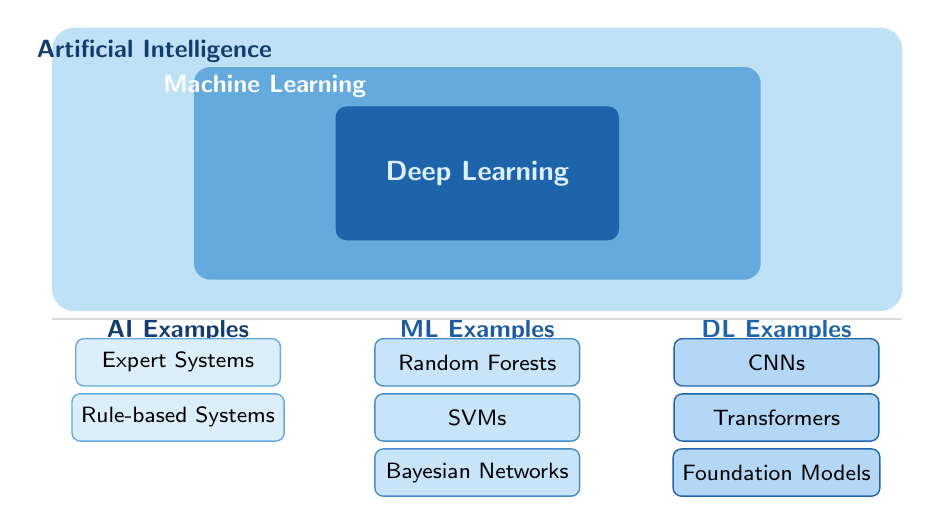
\begin{tikzpicture}[
    every node/.style={font=\small\sffamily},
    exbox/.style={
        rectangle, rounded corners=3pt,
        fill=white, draw=gray!50, line width=0.5pt,
        minimum width=2.6cm, minimum height=0.6cm,
        align=center, font=\footnotesize\sffamily
    },
    colhead/.style={font=\small\sffamily\bfseries, align=center}
]

%% ── Nested rectangles ──────────────────────────────────────────────
%% Outermost: Artificial Intelligence (light blue)
\fill[rounded corners=8pt,
      fill={rgb,255:red,190;green,225;blue,245}]
    (-5.4, 2.6) rectangle (5.4, -1.0);

%% Middle: Machine Learning (medium blue)
\fill[rounded corners=6pt,
      fill={rgb,255:red,100;green,170;blue,220}]
    (-3.6, 2.1) rectangle (3.6, -0.6);

%% Innermost: Deep Learning (dark blue)
\fill[rounded corners=4pt,
      fill={rgb,255:red,30;green,100;blue,170}]
    (-1.8, 1.6) rectangle (1.8, -0.1);

%% Labels inside each region
\node[text={rgb,255:red,220;green,240;blue,255},
      font=\normalsize\sffamily\bfseries]
    at (0, 0.75) {Deep Learning};

\node[text=white, font=\small\sffamily\bfseries]
    at (-2.7, 1.85) {Machine Learning};

\node[text={rgb,255:red,20;green,60;blue,110},
      font=\small\sffamily\bfseries]
    at (-4.1, 2.3) {Artificial Intelligence};

%% ── Example columns below ──────────────────────────────────────────
\def\rowA{-1.65}
\def\rowB{-2.35}
\def\rowC{-3.05}

%% Column headers
\node[colhead, text={rgb,255:red,20;green,60;blue,110}]
    at (-3.8, -1.25) {AI Examples};
\node[colhead, text={rgb,255:red,30;green,90;blue,160}]
    at (0,    -1.25) {ML Examples};
\node[colhead, text={rgb,255:red,30;green,100;blue,170}]
    at (3.8,  -1.25) {DL Examples};

%% AI column
\node[exbox, fill={rgb,255:red,220;green,238;blue,250},
      draw={rgb,255:red,100;green,170;blue,220}]
    at (-3.8, \rowA) {Expert Systems};
\node[exbox, fill={rgb,255:red,220;green,238;blue,250},
      draw={rgb,255:red,100;green,170;blue,220}]
    at (-3.8, \rowB) {Rule-based Systems};

%% ML column
\node[exbox, fill={rgb,255:red,200;green,228;blue,248},
      draw={rgb,255:red,70;green,140;blue,200}]
    at (0, \rowA) {Random Forests};
\node[exbox, fill={rgb,255:red,200;green,228;blue,248},
      draw={rgb,255:red,70;green,140;blue,200}]
    at (0, \rowB) {SVMs};
\node[exbox, fill={rgb,255:red,200;green,228;blue,248},
      draw={rgb,255:red,70;green,140;blue,200}]
    at (0, \rowC) {Bayesian Networks};

%% DL column
\node[exbox, fill={rgb,255:red,180;green,215;blue,245},
      draw={rgb,255:red,30;green,100;blue,170}]
    at (3.8, \rowA) {CNNs};
\node[exbox, fill={rgb,255:red,180;green,215;blue,245},
      draw={rgb,255:red,30;green,100;blue,170}]
    at (3.8, \rowB) {Transformers};
\node[exbox, fill={rgb,255:red,180;green,215;blue,245},
      draw={rgb,255:red,30;green,100;blue,170}]
    at (3.8, \rowC) {Foundation Models};

%% Thin separator line
\draw[gray!30, line width=0.4pt]
    (-5.4, -1.1) -- (5.4, -1.1);

\end{tikzpicture}

    \caption{Tassonomia dell'intelligenza artificiale come discipline annidate. L'apprendimento automatico (ML) è un sottoinsieme dell'IA; l'apprendimento profondo (DL) è un sottoinsieme del ML. Ogni dominio interno impiega approcci più orientati ai dati e all'apprendimento delle rappresentazioni rispetto al suo genitore. Sono indicati esempi di metodi all'interno di ciascun dominio.}
    \label{fig:ai_taxonomy}
\end{figure}

\subsection{Terminologia Chiave}

Precise use of terminology is essential for critical engagement with the AI literature. The following definitions are used consistently throughout this handbook:

\begin{description}
    \item[\textbf{Algoritmo}] Una sequenza finita e ordinata di istruzioni computazionali che trasforma un input in un output. Un algoritmo è la procedura; un modello è l'artefatto prodotto applicando tale procedura ai dati.

    \item[\textbf{Modello}] Una funzione matematica, parametrizzata da valori appresi dai dati, che mappa gli input (ad es., i valori dei pixel di un'immagine istologica) sugli output (ad es., una probabilità di malignià). Il modello codifica la conoscenza estratta durante l'addestramento.

    \item[\textbf{Addestramento}] Il processo mediante il quale i parametri di un modello vengono regolati, tipicamente minimizzando una funzione di perdita su un dataset etichettato, in modo che le previsioni del modello diventino sempre più accurate. L'addestramento è computazionalmente intensivo e viene eseguito una volta (o aggiornato periodicamente) prima del dispiegamento.

    \item[\textbf{Inferenza}] L'applicazione di un modello addestrato a nuovi dati non visti in precedenza per generare previsioni. L'inferenza è ciò che avviene nel dispiegamento clinico: il modello è fisso e i nuovi casi vengono passati attraverso di esso per ottenere output.

    \item[\textbf{Etichetta}] L'annotazione ground truth associata a un esempio di addestramento. Nell'apprendimento supervisionato, le etichette sono fornite da esperti umani (ad es., un patologo che annota una regione come ``carcinoma invasivo'' o ``epitelio normale''). La qualità e la coerenza delle etichette determinano direttamente la qualità del modello addestrato.

    \item[\textbf{Caratteristica}] Una proprietà o caratteristica misurabile dei dati di input utilizzata da un modello per fare previsioni. Nel ML classico, le caratteristiche sono progettate manualmente da esperti del dominio (ad es., area nucleare, texture della cromatina, rapporto ghiandola-stroma). Nell'apprendimento profondo, le caratteristiche vengono apprese automaticamente dai dati grezzi.
\end{description}

La comprensione di questi termini consente al professionista di leggere criticamente i lavori sull'IA, di interrogare le affermazioni dei fornitori sugli strumenti diagnostici basati sull'IA e di partecipare in modo significativo alla validazione e alla governance dei sistemi di IA all'interno del laboratorio.

% ============================================================
\section{IA Simbolica e Sistemi Basati su Regole}
\label{sec:ch3_symbolic}
% ============================================================

\subsection{Sistemi Esperti e Ragionamento Basato su Regole}

I primi sistemi di IA pratici in medicina erano \textbf{sistemi esperti}: programmi che codificavano la conoscenza di specialisti umani come un insieme strutturato di regole logiche, tipicamente nella forma \textit{SE} [condizione] \textit{ALLORA} [conclusione]. Il sistema MYCIN, sviluppato all'Università di Stanford negli anni Settanta per raccomandare la terapia antibiotica per le infezioni batteriche, è l'esempio canonico. I sistemi esperti sono composti da due componenti: una \textbf{base di conoscenza} contenente le regole specifiche del dominio, e un \textbf{motore di inferenza} che applica tali regole a un dato insieme di input per giungere a una conclusione. In patologia, i sistemi basati su regole sono stati implementati in software di analisi delle immagini per svolgere compiti come la segmentazione cellulare, la quantificazione della colorazione e la misurazione morfometrica.

Gli \textbf{alberi decisionali} sono un formalismo strettamente correlato in cui una serie di domande binarie sulle caratteristiche di input sono disposte in una struttura ad albero gerarchica. In ogni nodo interno, l'algoritmo verifica una caratteristica rispetto a una soglia; il risultato determina quale ramo viene seguito, fino a raggiungere un nodo foglia che specifica la classe o il valore previsto. Gli alberi decisionali sono intrinsecamente interpretabili: il percorso dalla radice alla foglia costituisce una spiegazione leggibile dall'uomo della previsione. Erano ampiamente utilizzati nei primi sistemi di diagnosi assistita da computer (CAD) e rimangono preziosi come componenti di metodi ensemble come le foreste casuali (Sezione~\ref{sec:ch3_ml}).

\subsection{La Valutazione del Ki-67 come Esempio di Analisi delle Immagini Basata su Regole}

Il Ki-67 è una proteina nucleare espressa nelle cellule in proliferazione e viene valutata di routine mediante immunoistochimica (IHC) nel cancro al seno per stimare l'indice di proliferazione — la proporzione di cellule tumorali che ciclano attivamente attraverso il ciclo cellulare. L'indice di proliferazione Ki-67 ha significato prognostico e predittivo: un'elevata espressione di Ki-67 è associata a un comportamento tumorale aggressivo e può influenzare le decisioni riguardanti la chemioterapia adiuvante \cite{bankhead2022}.

In un sistema di analisi delle immagini basato su regole, la valutazione del Ki-67 procede attraverso una sequenza deterministica di passaggi. In primo luogo, l'immagine viene convertita dallo spazio colore RGB standard a una rappresentazione con separazione delle colorazioni mediante deconvoluzione di Beer-Lambert, isolando il canale della diaminobenzidina (DAB) (marrone, indicante la positività al Ki-67) dal canale dell'ematossilina (blu, indicante tutti i nuclei). In secondo luogo, un algoritmo di segmentazione nucleare — tipicamente basato sulla sogliatura dell'intensità seguita dalla trasformata watershed — identifica i singoli nuclei come oggetti discreti. In terzo luogo, per ogni nucleo segmentato viene calcolata la densità ottica media del DAB. In quarto luogo, viene applicata una soglia: i nuclei con densità ottica media del DAB superiore a un valore definito (ad es., 0,2 unità di assorbanza) sono classificati come \textbf{positivi}; quelli al di sotto della soglia sono classificati come \textbf{negativi}. Infine, l'indice di proliferazione viene calcolato come:

\begin{equation}
    \text{Indice Ki-67} = \frac{N_{\text{positive}}}{N_{\text{positive}} + N_{\text{negative}}} \times 100\%
\end{equation}

dove $N_{\text{positive}}$ e $N_{\text{negative}}$ sono rispettivamente i conteggi dei nuclei DAB-positivi e DAB-negativi. L'intera procedura è implementata in piattaforme come QuPath \cite{bankhead2017}, dove la soglia e i parametri di segmentazione sono impostati dall'utente e applicati uniformemente all'immagine.

\subsection{Punti di Forza e Limitazioni dei Sistemi Basati su Regole}

I sistemi basati su regole offrono diversi vantaggi importanti. Sono \textbf{interpretabili}: ogni decisione può essere ricondotta a una regola specifica, rendendo il comportamento del sistema trasparente e verificabile. Sono \textbf{deterministici}: dato lo stesso input e le stesse regole, l'output è sempre identico, il che è essenziale per la riproducibilità in un contesto diagnostico. Sono anche \textbf{veloci} e computazionalmente poco costosi, non richiedendo dati di addestramento né hardware GPU. Per compiti ben definiti e vincolati — come il conteggio dei nuclei DAB-positivi in un preparato IHC colorato uniformemente — i sistemi basati su regole possono raggiungere prestazioni eccellenti e sono del tutto adeguati allo scopo.

Tuttavia, i sistemi basati su regole presentano limitazioni fondamentali che diventano evidenti quando il compito è più complesso o i dati più variabili. Sono \textbf{fragili}: piccole variazioni nel protocollo di colorazione, nella processazione tissutale o nella calibrazione dello scanner possono spostare la distribuzione della densità ottica del DAB, causando la classificazione errata dei nuclei da parte della soglia fissa. Sono \textbf{difficili da generalizzare}: un insieme di regole ottimizzato per il protocollo di colorazione Ki-67 di un laboratorio può avere prestazioni scadenti quando applicato a vetrini di un'istituzione diversa. \textbf{Non possono apprendere}: se le regole sono errate o incomplete, il sistema fallirà sistematicamente, e il miglioramento richiede la revisione manuale della base di conoscenza da parte di un esperto del dominio. Inoltre, i sistemi basati su regole sono poco adatti a compiti che richiedono l'integrazione di informazioni contestuali — ad esempio, distinguere i linfociti infiltranti il tumore dalle cellule tumorali in un campo densamente cellulare — perché tali distinzioni dipendono da relazioni spaziali e dal contesto morfologico che sono difficili da codificare come regole esplicite \cite{rashidi2019}.

Queste limitazioni hanno motivato lo sviluppo di approcci di apprendimento automatico, che possono adattare il loro comportamento alle proprietà statistiche dei dati di addestramento e generalizzare in modo più robusto in condizioni variabili.

% ============================================================
\section{Apprendimento Automatico: Approcci Supervisionati e Non Supervisionati}
\label{sec:ch3_ml}
% ============================================================

\subsection{Il Paradigma dell'Apprendimento Automatico}

L'apprendimento automatico rappresenta un cambiamento fondamentale nel modo in cui i sistemi computazionali vengono progettati. Invece di specificare le regole che governano il comportamento di un sistema, lo sviluppatore specifica un'\textbf{architettura del modello} (la forma matematica della funzione da apprendere) e un \textbf{algoritmo di apprendimento} (la procedura per regolare i parametri del modello), e poi espone il sistema ai dati da cui inferisce automaticamente le regole appropriate. Questo approccio basato sui dati consente ai sistemi ML di catturare relazioni complesse e non lineari in dati ad alta dimensionalità che sarebbero intrattabili da codificare manualmente \cite{komura2018}.

Il concetto centrale nel ML è il \textbf{vettore di caratteristiche}: una rappresentazione numerica di un esempio di input, costruita misurando un insieme di proprietà predefinite. Nell'analisi delle immagini istopatologiche, le caratteristiche possono includere area nucleare, perimetro, circolarità, intensità media della cromatina, descrittori di texture (ad es., caratteristiche di Haralick derivate dalla matrice di co-occorrenza dei livelli di grigio) e statistiche spaziali che descrivono la disposizione delle cellule all'interno di una regione tissutale. La qualità della rappresentazione delle caratteristiche è critica: se le caratteristiche non catturano le informazioni rilevanti per il compito, nessun algoritmo di apprendimento può compensare questa carenza. L'ingegneria delle caratteristiche — il processo di progettazione di caratteristiche informative — era storicamente un importante collo di bottiglia nel ML applicato alla patologia, richiedendo una profonda competenza nel dominio e un notevole sforzo manuale.

\subsection{Apprendimento Supervisionato}

Nell'\textbf{apprendimento supervisionato}, il modello viene addestrato su un dataset di coppie input-output $\{(\mathbf{x}_i, y_i)\}_{i=1}^{N}$, dove $\mathbf{x}_i$ è il vettore di caratteristiche dell'$i$-esimo esempio e $y_i$ è la sua etichetta. L'algoritmo di apprendimento regola i parametri del modello per minimizzare una \textbf{funzione di perdita} $\mathcal{L}(\hat{y}, y)$ che quantifica la discrepanza tra le previsioni del modello $\hat{y}$ e le etichette vere $y$. Esistono due tipi principali di compiti nell'apprendimento supervisionato:

\begin{itemize}
    \item \textbf{Classificazione}: L'output $y$ è una categoria discreta (ad es., ``maligno'' vs.\ ``benigno''; ``Grado 1'', ``Grado 2'', o ``Grado 3''). Le funzioni di perdita comuni includono la cross-entropy loss. Le prestazioni vengono valutate utilizzando metriche come accuratezza, sensibilità, specificità, area sotto la curva ROC (AUROC) e il punteggio F1.

    \item \textbf{Regressione}: L'output $y$ è un valore continuo (ad es., indice Ki-67 previsto, percentuale di cellularità tumorale o tempo di sopravvivenza del paziente). Le funzioni di perdita comuni includono l'errore quadratico medio (MSE) e l'errore assoluto medio (MAE).
\end{itemize}

La qualità dell'apprendimento supervisionato è fondamentalmente vincolata dalla qualità e dalla quantità dei dati di addestramento etichettati. Ottenere annotazioni di esperti per grandi dataset istopatologici è costoso e dispendioso in termini di tempo, e la variabilità inter-osservatore tra i patologi introduce rumore nelle etichette che può degradare le prestazioni del modello \cite{bera2019}.

\subsection{Apprendimento Non Supervisionato e Semi-Supervisionato}

L'\textbf{apprendimento non supervisionato} opera su dati non etichettati, cercando di scoprire strutture intrinseche — come cluster, varietà o fattori generativi — senza riferimento a categorie predefinite. Gli algoritmi di \textbf{clustering}, come $k$-means e il clustering agglomerativo gerarchico, partizionano i dati in gruppi di esempi simili. In patologia, il clustering non supervisionato è stato applicato per identificare sottotipi tumorali morfologicamente distinti, per stratificare i pazienti in base alla composizione del microambiente tissutale e per scoprire nuovi fenotipi istologici associati ad alterazioni molecolari. I metodi di riduzione della dimensionalità come l'analisi delle componenti principali (PCA) e la proiezione e approssimazione di varietà uniforme (UMAP) sono frequentemente utilizzati in combinazione con il clustering per visualizzare spazi di caratteristiche ad alta dimensionalità.

L'\textbf{apprendimento semi-supervisionato} occupa lo spazio tra gli approcci supervisionati e non supervisionati, sfruttando un piccolo dataset etichettato insieme a un dataset non etichettato molto più grande. Questo è particolarmente rilevante in patologia, dove le WSI non etichettate sono abbondanti ma le annotazioni di esperti sono scarse. I metodi semi-supervisionati utilizzano la struttura dei dati non etichettati — ad esempio, l'assunzione che i punti vicini nello spazio delle caratteristiche debbano avere la stessa etichetta — per regolarizzare il modello e migliorare la generalizzazione oltre quanto sarebbe ottenibile con i soli dati etichettati.

\subsection{Algoritmi Classici di Apprendimento Automatico}

Diversi algoritmi classici di ML rimangono ampiamente utilizzati nella ricerca in patologia e nelle applicazioni cliniche:

La \textbf{regressione logistica} è un modello lineare per la classificazione binaria che stima la probabilità di appartenenza a una classe come funzione sigmoide di una combinazione lineare delle caratteristiche di input. Nonostante la sua semplicità, la regressione logistica è robusta, interpretabile e funziona bene quando il confine decisionale è approssimativamente lineare nello spazio delle caratteristiche. Viene frequentemente utilizzata come modello di riferimento e per compiti in cui l'interpretabilità è fondamentale.

Le \textbf{macchine a vettori di supporto} (SVM) trovano l'iperpiano nello spazio delle caratteristiche che separa massimamente le due classi, massimizzando il margine tra gli esempi di addestramento più vicini (i vettori di supporto) e il confine decisionale. Le SVM possono essere estese alla classificazione non lineare attraverso il \textbf{kernel trick}, che mappa implicitamente i dati in uno spazio di dimensionalità superiore dove la separazione lineare è possibile. Le SVM erano l'approccio dominante nella patologia computazionale negli anni Duemila e all'inizio degli anni Duemiladieci, raggiungendo prestazioni elevate in compiti come il rilevamento delle mitosi e la classificazione tumorale.

Le \textbf{foreste casuali} sono metodi ensemble che costruiscono un gran numero di alberi decisionali, ciascuno addestrato su un campione bootstrap casuale dei dati di addestramento e utilizzando un sottoinsieme casuale di caratteristiche ad ogni divisione. La previsione finale si ottiene per voto di maggioranza (classificazione) o mediando (regressione) su tutti gli alberi. Le foreste casuali sono robuste all'overfitting, gestiscono bene gli spazi di caratteristiche ad alta dimensionalità e forniscono una misura naturale dell'importanza delle caratteristiche, rendendole preziose sia per la previsione che per l'analisi esplorativa \cite{rashidi2019}.

\subsection{Overfitting, Regolarizzazione e Validazione Incrociata}

Una sfida centrale nel ML è l'\textbf{overfitting}: la tendenza di un modello a memorizzare i dati di addestramento, inclusi il loro rumore e le loro idiosincrasie, piuttosto che apprendere il pattern generalizzabile sottostante. Un modello in overfitting raggiunge un'elevata accuratezza sul set di addestramento ma ha prestazioni scadenti su nuovi dati non visti. L'overfitting è più probabile quando il modello è complesso (molti parametri) rispetto alla dimensione del dataset di addestramento.

Le tecniche di \textbf{regolarizzazione} mitigano l'overfitting penalizzando la complessità del modello. La regolarizzazione L1 (Lasso) aggiunge una penale proporzionale alla somma dei valori assoluti dei parametri del modello, incoraggiando soluzioni sparse. La regolarizzazione L2 (Ridge) aggiunge una penale proporzionale alla somma dei parametri al quadrato, riducendo tutti i parametri verso zero. Il dropout, utilizzato nelle reti neurali, disattiva casualmente una proporzione di neuroni durante l'addestramento, prevenendo la co-adattazione.

La \textbf{validazione incrociata} è la metodologia standard per stimare le prestazioni di generalizzazione di un modello. Nella validazione incrociata a $k$ fold, il dataset viene partizionato in $k$ sottoinsiemi uguali (fold); il modello viene addestrato su $k-1$ fold e valutato sul fold trattenuto, e questo processo viene ripetuto $k$ volte in modo che ogni esempio serva come caso di test esattamente una volta. La media e la deviazione standard delle prestazioni tra i fold forniscono una stima imparziale delle prestazioni di generalizzazione. In patologia, è fondamentale che le divisioni della validazione incrociata vengano eseguite a livello di paziente (non a livello di immagine o patch) per prevenire la fuga di dati, in cui le informazioni dello stesso paziente compaiono sia nel set di addestramento che in quello di test.

% ============================================================
\section{Reti Bayesiane e Ragionamento Probabilistico}
\label{sec:ch3_bayesian}
% ============================================================

\subsection{Inferenza Bayesiana}

L'inferenza bayesiana fornisce un quadro matematico rigoroso per aggiornare le credenze alla luce delle prove. Si basa sul \textbf{teorema di Bayes}:

\begin{equation}
    P(H \mid E) = \frac{P(E \mid H) \cdot P(H)}{P(E)}
\end{equation}

dove $H$ è un'ipotesi (ad es., ``la lesione è maligna''), $E$ è la prova osservata (ad es., i risultati di un pannello di colorazioni immunoistochimiche), $P(H)$ è la \textbf{probabilità a priori} dell'ipotesi prima che la prova venga considerata, $P(E \mid H)$ è la \textbf{verosimiglianza} di osservare la prova dato che l'ipotesi è vera, $P(H \mid E)$ è la \textbf{probabilità a posteriori} dell'ipotesi dopo aver incorporato la prova, e $P(E)$ è la probabilità marginale della prova (una costante di normalizzazione). In patologia diagnostica, la probabilità a priori corrisponde alla probabilità pre-test di una diagnosi dato il contesto clinico (età del paziente, sesso, sede della biopsia, risultati dell'imaging), e la probabilità a posteriori è la probabilità aggiornata dopo che i risultati istologici e ancillari sono stati incorporati.

Il quadro bayesiano è particolarmente adatto al ragionamento diagnostico perché modella esplicitamente l'incertezza. Invece di produrre una singola diagnosi deterministica, un sistema bayesiano produce una distribuzione di probabilità sulle possibili diagnosi, quantificando il grado di fiducia in ciascuna. Questo è clinicamente prezioso: un sistema che riporta ``probabilità di carcinoma sieroso ad alto grado: 0,87; probabilità di carcinoma endometrioide: 0,11; probabilità di carcinoma a cellule chiare: 0,02'' trasmette informazioni più utili di una classificazione binaria, e consente al clinico di calibrare la propria risposta in modo appropriato.

\subsection{Reti Bayesiane}

Una \textbf{rete bayesiana} (BN) è un modello grafico probabilistico che rappresenta un insieme di variabili e le loro dipendenze condizionali come un \textbf{grafo aciclico diretto} (DAG). Ogni nodo nel grafo rappresenta una variabile casuale (ad es., un reperto clinico, una caratteristica istologica o una diagnosi), e ogni arco diretto rappresenta una dipendenza condizionale tra variabili. L'assenza di un arco tra due nodi codifica l'assunzione di indipendenza condizionale, che consente di fattorizzare la distribuzione di probabilità congiunta su tutte le variabili in un prodotto di distribuzioni di probabilità condizionali locali — una per ogni nodo dati i suoi genitori nel grafo.

In una rete bayesiana diagnostica per la patologia mammaria, ad esempio, i nodi potrebbero rappresentare variabili come l'età del paziente, il grado tumorale, lo stato del recettore degli estrogeni (ER), lo stato del recettore del progesterone (PR), lo stato HER2, l'indice Ki-67 e la presenza di invasione linfovascolare. Gli archi codificano le dipendenze biologiche e statistiche note: ad esempio, lo stato ER influenza lo stato PR, ed entrambi influenzano la probabilità di risposta alla terapia endocrina. Dati i valori osservati per un sottoinsieme di nodi (la prova), la rete può calcolare la distribuzione di probabilità a posteriori su tutti i nodi non osservati utilizzando algoritmi di inferenza esatta o approssimata.

\subsection{Vantaggi e Limitazioni nel Supporto Decisionale Diagnostico}

Le reti bayesiane offrono diversi vantaggi per il supporto decisionale diagnostico in patologia. In primo luogo, forniscono \textbf{quantificazione dell'incertezza}: l'output è una distribuzione di probabilità, non una stima puntuale, rendendo esplicita la fiducia del sistema. In secondo luogo, sono \textbf{interpretabili}: la struttura del grafo codifica la conoscenza del dominio in una forma che i clinici possono ispezionare e validare. In terzo luogo, possono \textbf{gestire i dati mancanti} in modo elegante: se un particolare risultato di test non è disponibile, la rete marginalizza sulla variabile mancante invece di fallire. In quarto luogo, possono \textbf{incorporare la conoscenza a priori}: la struttura e i parametri iniziali della rete possono essere specificati da esperti del dominio e poi raffinati utilizzando i dati, combinando i punti di forza degli approcci basati sulla conoscenza e basati sui dati.

Le principali limitazioni delle reti bayesiane sono la loro \textbf{scalabilità} e la loro \textbf{assunzione di indipendenza condizionale}. All'aumentare del numero di variabili, il numero di parametri necessari per specificare le tabelle di probabilità condizionale cresce esponenzialmente, rendendo l'inferenza esatta computazionalmente intrattabile per reti di grandi dimensioni. I metodi di inferenza approssimata (ad es., Monte Carlo a catena di Markov, inferenza variazionale) possono affrontare questo problema, ma a costo di una complessità aggiuntiva. Inoltre, le assunzioni di indipendenza condizionale codificate nella struttura del grafo potrebbero non valere in pratica, e la specificazione errata del grafo può portare a un'inferenza distorta. Nonostante queste limitazioni, le reti bayesiane sono state applicate con successo al supporto decisionale diagnostico in oncologia, radiologia e patologia, e rimangono un'area di ricerca attiva \cite{rashidi2019}.

% ============================================================
\section{Dalle Caratteristiche alle Rappresentazioni: Il Passaggio all'Apprendimento Profondo}
\label{sec:ch3_deeplearning}
% ============================================================

\subsection{Le Limitazioni delle Caratteristiche Costruite Manualmente}

Gli approcci classici di ML in patologia dipendono criticamente dalla qualità delle caratteristiche costruite manualmente utilizzate per rappresentare le immagini. La progettazione di caratteristiche informative richiede una profonda competenza nel dominio, è dispendiosa in termini di tempo ed è intrinsecamente limitata dalla conoscenza pregressa del progettista su ciò che è diagnosticamente rilevante. Le caratteristiche efficaci per un compito (ad es., la morfometria nucleare per la classificazione) possono essere non informative per un altro (ad es., la predizione dell'instabilità dei microsatelliti dalla morfologia E\&E). Inoltre, le caratteristiche costruite manualmente vengono tipicamente calcolate da singole cellule o piccole regioni di interesse, e possono non riuscire a catturare l'organizzazione spaziale del tessuto a più scale — la disposizione delle ghiandole, la composizione del microambiente tumorale, la relazione tra tumore e stroma — che è sempre più riconosciuta come diagnosticamente e prognosticamente importante \cite{bera2019}.

L'intuizione fondamentale dell'apprendimento profondo è che, dati dati sufficienti e risorse computazionali, una rete neurale può \textbf{apprendere} la rappresentazione ottimale delle caratteristiche per un dato compito direttamente dai dati grezzi dei pixel, senza alcuna ingegneria manuale delle caratteristiche. Le caratteristiche apprese non sono interpretabili allo stesso modo delle misurazioni morfometriche costruite manualmente, ma possono catturare pattern complessi e non lineari che sono invisibili all'ingegneria convenzionale delle caratteristiche. Questo passaggio dall'ingegneria delle caratteristiche all'\textbf{apprendimento delle rappresentazioni} è la caratteristica distintiva della rivoluzione dell'apprendimento profondo nella patologia computazionale \cite{song2023}.

\subsection{Reti Neurali Artificiali}

Una \textbf{rete neurale artificiale} (ANN) è un modello computazionale liberamente ispirato alla struttura dei circuiti neurali biologici. È composta da una serie di \textbf{strati}, ciascuno comprendente un insieme di unità computazionali chiamate \textbf{neuroni} (o nodi). Ogni neurone calcola una somma pesata dei suoi input, aggiunge un termine di bias e passa il risultato attraverso una \textbf{funzione di attivazione} non lineare per produrre il suo output. Le funzioni di attivazione comuni includono l'unità lineare rettificata (ReLU, $f(x) = \max(0, x)$), la funzione sigmoide ($f(x) = 1/(1+e^{-x})$) e la tangente iperbolica (tanh). La non linearità della funzione di attivazione è essenziale: senza di essa, una rete multistrato sarebbe matematicamente equivalente a una singola trasformazione lineare, indipendentemente dalla sua profondità.

Una rete con uno o più \textbf{strati nascosti} tra gli strati di input e output è chiamata \textbf{percettrone multistrato} (MLP). La \textbf{profondità} di una rete si riferisce al numero di strati; le reti profonde (con molti strati) possono rappresentare funzioni dell'input sempre più astratte e complesse. I parametri della rete — i pesi e i bias di tutti i neuroni — vengono appresi durante l'addestramento mediante \textbf{backpropagation}: il gradiente della funzione di perdita rispetto a ciascun parametro viene calcolato usando la regola della catena del calcolo, e i parametri vengono aggiornati nella direzione che riduce la perdita, utilizzando un algoritmo di ottimizzazione come la discesa del gradiente stocastica (SGD) o Adam.

\subsection{Reti Neurali Convoluzionali per l'Analisi delle Immagini}

Per i compiti di analisi delle immagini, l'architettura di rete neurale più importante è la \textbf{rete neurale convoluzionale} (CNN). Le CNN sfruttano la struttura spaziale delle immagini attraverso due operazioni chiave. Prima, la \textbf{convoluzione}: un piccolo filtro (kernel) di pesi apprendibili viene fatto scorrere sull'immagine, calcolando il prodotto scalare tra il filtro e ogni patch locale di pixel. Questo produce una \textbf{mappa delle caratteristiche} che codifica la presenza e la posizione di un particolare pattern (ad es., un bordo, una texture o un motivo più complesso) nell'immagine. Più filtri vengono applicati in parallelo, producendo più mappe delle caratteristiche. Seconda, il \textbf{pooling}: le mappe delle caratteristiche vengono sottocampionate spazialmente (ad es., prendendo il valore massimo in ogni regione $2 \times 2$ non sovrapposta), riducendo la risoluzione spaziale mantenendo le attivazioni più salienti e introducendo un grado di invarianza alla traslazione.

Impilando più strati convoluzionali e di pooling, una CNN costruisce una rappresentazione gerarchica dell'immagine: gli strati iniziali rilevano caratteristiche di basso livello come bordi e gradienti di colore; gli strati intermedi rilevano caratteristiche di medio livello come texture e forme; e gli strati profondi rilevano caratteristiche di alto livello, semanticamente significative, come strutture ghiandolari, pleomorfismo nucleare o figure mitotiche. Questo apprendimento gerarchico delle caratteristiche è ciò che rende le CNN così potenti per l'analisi delle immagini istopatologiche \cite{komura2018}. Architetture come ResNet, VGG, Inception ed EfficientNet, originariamente sviluppate per il riconoscimento di immagini naturali, sono state ampiamente adattate e ottimizzate per applicazioni in patologia, spesso utilizzando il \textbf{transfer learning}: inizializzando la rete con pesi pre-addestrati su un grande dataset di immagini naturali (ad es., ImageNet) e poi ottimizzando su un dataset più piccolo specifico per la patologia.

\subsection{Oltre le CNN: Transformer e Modelli Fondazionali}

Più recentemente, i \textbf{vision transformer} (ViT) e i \textbf{modelli fondazionali} sono emersi come potenti alternative alle CNN per la patologia computazionale. I transformer, originariamente sviluppati per l'elaborazione del linguaggio naturale, utilizzano un meccanismo di \textbf{auto-attenzione} che consente a ogni elemento dell'input (ad es., ogni patch di una WSI) di prestare attenzione a tutti gli altri elementi, catturando dipendenze spaziali a lungo raggio che sono difficili da modellare per le CNN. I modelli fondazionali — grandi reti neurali pre-addestrate su dataset massicci e diversificati mediante apprendimento auto-supervisionato — possono essere ottimizzati per un'ampia gamma di compiti a valle con relativamente pochi dati etichettati. Modelli come UNI, CONCH e PLIP, pre-addestrati su milioni di immagini patologiche, rappresentano la frontiera attuale del settore e stanno iniziando a dimostrare prestazioni che si avvicinano o superano quelle dei patologi specialisti in una serie di compiti diagnostici \cite{song2023}.

% ============================================================
\section{Il Ruolo del Tecnico nei Processi Assistiti dall'IA}
\label{sec:ch3_technician}
% ============================================================

\subsection{L'Imperativo dell'Uomo nel Ciclo}

Il dispiegamento dell'IA in patologia clinica non elimina la necessità di competenza umana; piuttosto, trasforma e per certi aspetti eleva il ruolo del tecnico di laboratorio biomedico. I sistemi di IA sono strumenti, e come tutti gli strumenti possono fallire — a volte in modi sottili, sistematici e difficili da rilevare senza conoscenza del dominio. Il concetto di \textbf{uomo nel ciclo} (HITL) si riferisce all'integrazione del giudizio umano in punti critici di un flusso di lavoro assistito dall'IA, garantendo che gli output del sistema vengano esaminati, validati e contestualizzati da un professionista competente prima che influenzino le decisioni cliniche \cite{bankhead2022}. Il tecnico che comprende i principi alla base di un sistema di IA è molto meglio attrezzato per identificarne le modalità di fallimento rispetto a chi lo tratta come una scatola nera.

\subsection{Annotazione dei Dati}

Le prestazioni di qualsiasi modello ML supervisionato sono fondamentalmente determinate dalla qualità dei suoi dati di addestramento, e la qualità dei dati di addestramento è fondamentalmente determinata dalla qualità delle sue annotazioni. L'\textbf{annotazione dei dati} — il processo di assegnazione di etichette agli esempi di addestramento — è un compito qualificato che richiede competenza nel dominio, attenzione ai dettagli e consapevolezza delle fonti di variabilità e ambiguità nelle immagini istopatologiche. I tecnici e i biologi di laboratorio biomedico sono sempre più coinvolti nei flussi di lavoro di annotazione, lavorando a fianco dei patologi per etichettare cellule, regioni di interesse, compartimenti tissutali e categorie diagnostiche in grandi dataset di immagini.

Le migliori pratiche nell'annotazione includono l'uso di linee guida di annotazione chiare e operativamente definite; sessioni di calibrazione regolari per valutare e minimizzare la variabilità inter-annotatore; l'uso di più annotatori indipendenti per i casi ambigui, con i disaccordi risolti per consenso o da un patologo senior; e il mantenimento di registri di provenienza dettagliati che documentano chi ha annotato ogni caso, quando e secondo quale versione delle linee guida. La qualità dell'annotazione dovrebbe essere monitorata continuamente, e i casi con elevato disaccordo inter-annotatore dovrebbero essere segnalati per la revisione. L'investimento in annotazioni di alta qualità non è semplicemente una questione tecnica: è il fondamento su cui si basa la validità clinica del modello di IA risultante.

\subsection{Controllo Qualità dei Dati di Addestramento e degli Output dell'IA}

Oltre all'annotazione, i tecnici svolgono un ruolo critico nel \textbf{controllo qualità} (QC) dei dati di addestramento. Le fonti comuni di problemi di qualità dei dati nella patologia digitale includono: artefatti di processazione tissutale (ad es., pieghe, lacerazioni, bolle d'aria, fissazione eccessiva o insufficiente); variabilità della colorazione (ad es., variazione da lotto a lotto nell'intensità dell'ematossilina ed eosina); artefatti di scansione (ad es., errori di messa a fuoco, artefatti di cucitura, polvere sul vetro dello scanner); ed errori di metadati (ad es., identificatori di caso errati, diagnosi etichettate erroneamente). Ciascuno di questi può introdurre bias sistematici in un modello addestrato. Una rigorosa pipeline di QC dovrebbe esaminare le immagini di addestramento per questi artefatti prima che entrino nel dataset di addestramento, e dovrebbe documentare i criteri di esclusione applicati.

Il controllo qualità degli output dell'IA nel dispiegamento clinico è ugualmente importante. I tecnici dovrebbero essere addestrati a riconoscere le modalità di fallimento caratteristiche dei sistemi di IA che utilizzano: ad esempio, un algoritmo di quantificazione del Ki-67 può sovrastimare i nuclei nelle regioni di piega tissutale, o può classificare erroneamente le cellule stromali come cellule tumorali nelle aree di desmoplasia. I controlli QC di routine — come l'ispezione visiva di un campione casuale di casi elaborati dall'IA, il confronto degli output dell'IA con i conteggi manuali su un sottoinsieme di casi e il monitoraggio delle distribuzioni degli output per spostamenti inattesi — sono salvaguardie essenziali. Qualsiasi discrepanza sistematica tra gli output dell'IA e la valutazione degli esperti dovrebbe essere segnalata e indagata.

\subsection{Validazione e Considerazioni Normative}

Prima che uno strumento di IA venga introdotto nella pratica clinica, deve essere rigorosamente validato su dati rappresentativi della popolazione di utilizzo prevista e che non sono stati utilizzati nell'addestramento. Gli studi di validazione dovrebbero valutare non solo le metriche di prestazione complessive (ad es., AUROC, sensibilità, specificità) ma anche le prestazioni tra sottogruppi clinicamente rilevanti (ad es., diversi sottotipi tumorali, diverse caratteristiche demografiche dei pazienti, diversi protocolli di colorazione) per identificare potenziali disparità. Il ruolo del tecnico nella validazione include la preparazione del dataset di validazione, l'esecuzione del sistema di IA sui casi di validazione, la registrazione degli output e il loro confronto con lo standard di riferimento stabilito dai patologi esperti.

I quadri normativi per i dispositivi diagnostici in vitro (IVD) basati sull'IA si stanno evolvendo rapidamente. Nell'Unione Europea, gli strumenti diagnostici basati sull'IA sono regolamentati dal Regolamento sui Dispositivi Diagnostici In Vitro (IVDR, UE 2017/746) e, ove applicabile, dall'AI Act (UE 2024/1689). Negli Stati Uniti, la FDA regola il software basato su IA/ML come dispositivo medico (SaMD) nell'ambito di un quadro che include disposizioni per i sistemi di apprendimento continuo. I tecnici dovrebbero essere consapevoli dello stato normativo degli strumenti di IA che utilizzano, delle condizioni in cui tali strumenti sono stati validati e degli obblighi del laboratorio riguardo alla sorveglianza post-commercializzazione e alla segnalazione degli incidenti \cite{bankhead2022}.

\subsection{Comprensione delle Limitazioni dell'IA}

Una competenza critica per qualsiasi professionista che lavora con l'IA è la capacità di riconoscere e articolare le limitazioni dei sistemi che utilizza. Le principali limitazioni di cui essere consapevoli includono:

\begin{itemize}
    \item \textbf{Spostamento della distribuzione}: I modelli di IA funzionano meglio su dati che assomigliano ai loro dati di addestramento. Quando la distribuzione degli input cambia — ad esempio, a causa di un cambiamento nel protocollo di colorazione, un nuovo modello di scanner o una diversa popolazione di pazienti — le prestazioni del modello possono degradarsi, a volte drasticamente, senza alcun segnale di avvertimento ovvio.

    \item \textbf{Apprendimento di scorciatoie}: I modelli possono imparare a sfruttare correlazioni spurie nei dati di addestramento (ad es., un particolare artefatto di colorazione che si trova a co-occorrere con una diagnosi nel set di addestramento) piuttosto che le vere caratteristiche diagnostiche. Tali scorciatoie potrebbero non essere evidenti dalle metriche di prestazione aggregate ma possono causare errori sistematici nel dispiegamento.

    \item \textbf{Calibrazione}: Le probabilità previste da un modello potrebbero non riflettere accuratamente la vera frequenza del risultato previsto. Un modello ben calibrato che prevede una probabilità del 70\% di malignià dovrebbe essere corretto circa il 70\% delle volte; un modello mal calibrato può essere sistematicamente troppo o troppo poco fiducioso.

    \item \textbf{Spiegabilità}: Molti modelli di apprendimento profondo sono difficili da interpretare: non è sempre possibile capire perché un modello ha fatto una particolare previsione. I metodi di spiegabilità come la mappatura dell'attivazione di classe pesata dal gradiente (Grad-CAM) e la visualizzazione dell'attenzione possono fornire una comprensione parziale, ma dovrebbero essere interpretati con cautela.
\end{itemize}

% ============================================================
\section{Attività Pratiche}
\label{sec:ch3_practical}
% ============================================================

\subsection{Attività 3.1: L'IA Simbolica in Azione --- Quantificazione del Ki-67 con QuPath}

\textbf{Obiettivo:} Dimostrare i principi dell'IA simbolica basata su regole implementando un algoritmo di rilevamento delle cellule positive al Ki-67 basato su soglia in QuPath \cite{bankhead2017}, ed esplorare la sensibilità del risultato alla scelta del parametro di soglia.

\textbf{Risultati di Apprendimento:} Al completamento di questa attività, gli studenti saranno in grado di: (1) spiegare i passaggi di una pipeline di analisi delle immagini basata su regole per la quantificazione IHC; (2) implementare un algoritmo di rilevamento delle cellule positive in QuPath utilizzando il classificatore basato su soglia integrato; (3) valutare criticamente l'effetto delle scelte dei parametri sull'indice Ki-67; e (4) identificare i tipi di errore prodotti dall'algoritmo e collegarli alle limitazioni dei sistemi basati su regole discusse nella Sezione~\ref{sec:ch3_symbolic}.

\textbf{Materiali Necessari:}
\begin{itemize}
    \item Un computer con QuPath (versione 0.4 o successiva) installato (disponibile gratuitamente da \url{https://qupath.github.io}).
    \item Un'immagine di vetrino intero di cancro al seno colorata con Ki-67 digitalizzata o una regione di interesse rappresentativa (fornita dal coordinatore del corso, o scaricabile dal repository di immagini campione di QuPath).
    \item La guida utente di QuPath (disponibile online).
\end{itemize}

\textbf{Procedura:}

\begin{enumerate}
    \item \textbf{Aprire l'immagine in QuPath.} Avviare QuPath e aprire la WSI Ki-67 o il tile di immagine fornito. Esaminare l'immagine a più ingrandimenti per familiarizzare con il pattern di colorazione: i nuclei DAB-positivi (marroni) sono cellule in proliferazione Ki-67-positive; i nuclei positivi all'ematossilina (blu) sono Ki-67-negativi.

    \item \textbf{Definire una regione di interesse (ROI).} Utilizzando lo strumento di annotazione rettangolo o poligono, disegnare una ROI che comprenda un'area rappresentativa del tumore invasivo, evitando necrosi, pieghe tissutali e aree di scarsa qualità della colorazione. Questo passaggio rispecchia la pratica del patologo di selezionare un ``hot spot'' o un'area rappresentativa per la valutazione del Ki-67.

    \item \textbf{Eseguire la stima del vettore di colorazione.} Navigare su \texttt{Analyze > Preprocessing > Estimate stain vectors}. QuPath stimerà automaticamente i vettori di colorazione dell'ematossilina e del DAB dall'immagine utilizzando un algoritmo di deconvoluzione del colore. Ispezionare i vettori stimati e regolarli se necessario per garantire una separazione accurata delle colorazioni.

    \item \textbf{Eseguire l'algoritmo di Rilevamento delle Cellule Positive.} Navigare su \texttt{Analyze > Cell detection > Positive cell detection}. Nella finestra di dialogo dei parametri, impostare quanto segue: \textit{Detection image}: ``Optical density sum''; \textit{Requested pixel size}: 0,5\,$\mu$m; \textit{Background radius}: 8\,$\mu$m; \textit{Median filter radius}: 0\,$\mu$m; \textit{Sigma}: 1,5\,$\mu$m; \textit{Minimum area}: 10\,$\mu$m$^2$; \textit{Maximum area}: 400\,$\mu$m$^2$. Per la soglia di positività, iniziare con una soglia OD media DAB di \textbf{0,2}. Fare clic su \textit{Run}.

    \item \textbf{Ispezionare i risultati.} QuPath sovrapporrà marcatori colorati su ogni nucleo rilevato: le cellule positive sono contrassegnate con un colore (tipicamente marrone o rosso) e le cellule negative con un altro (tipicamente blu). Aprire il pannello \textit{Annotations} per visualizzare le statistiche di riepilogo, incluso il conteggio totale delle cellule, il conteggio delle cellule positive e l'indice Ki-67 (espresso come percentuale).

    \item \textbf{Variare la soglia.} Ripetere l'analisi con soglie OD media DAB di \textbf{0,1} e \textbf{0,4}. Registrare l'indice Ki-67 ottenuto a ciascuna soglia. Notare come la classificazione dei nuclei borderline cambia al variare della soglia.

    \item \textbf{Identificare gli errori.} A ciascuna impostazione di soglia, ispezionare visivamente i risultati del rilevamento e identificare esempi di: (a) falsi positivi — cellule non tumorali (ad es., fibroblasti stromali, cellule endoteliali, linfociti) classificate come cellule tumorali Ki-67-positive; (b) falsi negativi — cellule tumorali Ki-67-positive mancate dall'algoritmo; (c) errori di segmentazione — nuclei che sono fusi (sotto-segmentati) o divisi (sovra-segmentati).
\end{enumerate}

\textbf{Domande di Discussione:}
\begin{enumerate}
    \item Come cambia l'indice Ki-67 al variare della soglia DAB? Quali sono le implicazioni cliniche di questa sensibilità?
    \item Quali tipi di errore sono più comuni a una soglia bassa rispetto a una soglia alta? Come si relazionano questi ai concetti di sensibilità e specificità?
    \item L'algoritmo non distingue tra cellule tumorali e cellule non tumorali. Come potrebbe questa limitazione influenzare la validità clinica dell'indice Ki-67 che produce? Come potrebbe essere affrontata questa limitazione utilizzando un approccio più sofisticato (ad es., basato sull'apprendimento automatico)?
    \item Confrontare l'indice Ki-67 prodotto dall'algoritmo con una stima visiva effettuata esaminando l'immagine manualmente. Quali sono le fonti di discrepanza?
    \item Riflettere sul ruolo del tecnico in questo flusso di lavoro. Quali decisioni richiedono il giudizio umano e quali sono le conseguenze degli errori in ogni punto decisionale?
\end{enumerate}

\textbf{Risultati Attesi e Interpretazione:} Gli studenti dovrebbero osservare che l'indice Ki-67 è sensibile alla scelta della soglia, con soglie più basse che producono indici più alti (più nuclei classificati come positivi) e soglie più alte che producono indici più bassi. La soglia ottimale non è universale ma dipende dal protocollo di colorazione, dallo scanner e dal tipo di tessuto. Questo esercizio illustra la limitazione fondamentale dei sistemi basati su regole: le loro prestazioni dipendono dalla corretta specificazione dei parametri che devono essere impostati da un esperto umano e potrebbero non generalizzarsi in diverse condizioni di laboratorio. Illustra anche il valore di tali sistemi per la quantificazione riproducibile e ad alto rendimento all'interno di un contesto definito e validato.

% ============================================================
\section{Sintesi}
\label{sec:ch3_summary}
% ============================================================

Questo capitolo ha fornito un'introduzione sistematica ai principi dell'intelligenza artificiale applicati alla patologia diagnostica. I seguenti punti chiave dovrebbero essere ricordati:

\begin{itemize}
    \item \textbf{L'IA è un campo ampio} che comprende qualsiasi sistema computazionale che esibisce un comportamento intelligente. In patologia clinica, tutte le attuali applicazioni di IA sono IA ristretta: altamente capaci all'interno di un dominio definito ma incapaci di generalizzare oltre di esso.

    \item \textbf{La tassonomia dell'IA} è gerarchica: l'apprendimento automatico è un sotto-campo dell'IA, e l'apprendimento profondo è un sotto-campo dell'apprendimento automatico. Comprendere questa gerarchia è essenziale per interpretare le affermazioni sugli strumenti diagnostici basati sull'IA.

    \item \textbf{L'IA simbolica e i sistemi basati su regole} codificano la conoscenza del dominio come regole logiche esplicite. Sono interpretabili, deterministici e computazionalmente efficienti, ma fragili e difficili da generalizzare. L'algoritmo basato su soglia Ki-67 in QuPath è un esempio paradigmatico.

    \item \textbf{L'apprendimento automatico} consente ai sistemi di apprendere dai dati piuttosto che da regole esplicite. L'apprendimento supervisionato (classificazione e regressione), l'apprendimento non supervisionato (clustering) e l'apprendimento semi-supervisionato hanno ciascuno applicazioni distinte in patologia. Gli algoritmi classici — regressione logistica, SVM, foreste casuali — rimangono ampiamente utilizzati. L'overfitting, la regolarizzazione e la validazione incrociata sono preoccupazioni metodologiche centrali.

    \item \textbf{Le reti bayesiane} forniscono un quadro rigoroso per il ragionamento diagnostico probabilistico, quantificando esplicitamente l'incertezza e incorporando la conoscenza clinica a priori. Sono particolarmente preziose per il supporto decisionale in scenari diagnostici complessi e multi-variabili.

    \item \textbf{L'apprendimento profondo} supera le limitazioni delle caratteristiche costruite manualmente apprendendo rappresentazioni gerarchiche direttamente dai dati grezzi delle immagini. Le reti neurali convoluzionali sono l'architettura dominante per l'analisi delle immagini istopatologiche, e i modelli fondazionali rappresentano la frontiera attuale del settore.

    \item \textbf{Il ruolo del tecnico} nella patologia assistita dall'IA è critico e multiforme: comprende l'annotazione dei dati, il controllo qualità dei dati di addestramento e degli output dell'IA, la validazione dei sistemi di IA e l'esercizio di un giudizio umano informato come salvaguardia contro gli errori dell'IA. La comprensione dei principi dell'IA è un prerequisito per svolgere questo ruolo in modo efficace.
\end{itemize}

% ============================================================
\section{Domande di Revisione}
\label{sec:ch3_questions}
% ============================================================

Le seguenti domande a risposta multipla sono progettate per consolidare la comprensione del materiale presentato in questo capitolo. Per ciascuna domanda, selezionare la singola risposta migliore.

\begin{enumerate}

    % Q1
    \item \label{ch3:q1} Quale delle seguenti affermazioni descrive meglio la relazione tra intelligenza artificiale, apprendimento automatico e apprendimento profondo?
    \begin{enumerate}[label=\Alph*.]
        \item Sono tre campi indipendenti e non correlati dell'informatica.
        \item L'apprendimento automatico è un sottoinsieme dell'apprendimento profondo, che è un sottoinsieme dell'intelligenza artificiale.
        \item L'apprendimento profondo è un sottoinsieme dell'apprendimento automatico, che è un sottoinsieme dell'intelligenza artificiale.
        \item L'intelligenza artificiale è un sottoinsieme dell'apprendimento automatico, che è un sottoinsieme dell'apprendimento profondo.
    \end{enumerate}

    % Q2
    \item \label{ch3:q2} Nel contesto dell'apprendimento automatico, quale delle seguenti definizioni descrive meglio un'\textit{etichetta}?
    \begin{enumerate}[label=\Alph*.]
        \item Una rappresentazione numerica dei dati di input utilizzata dal modello per effettuare previsioni.
        \item L'annotazione di riferimento assegnata a un esempio di addestramento da un esperto del dominio.
        \item La probabilità di output prodotta da un modello addestrato durante l'inferenza.
        \item Un parametro di regolarizzazione che controlla la complessità del modello.
    \end{enumerate}

    % Q3
    \item \label{ch3:q3} Un sistema di analisi delle immagini basato su regole per la valutazione del Ki-67 classifica un nucleo come positivo se la sua densità ottica media del DAB supera una soglia definita. Quale delle seguenti è la limitazione più significativa di questo approccio?
    \begin{enumerate}[label=\Alph*.]
        \item È computazionalmente troppo lento per l'uso routinario in laboratorio.
        \item Richiede un grande insieme di dati di addestramento etichettati per funzionare correttamente.
        \item La soglia fissa potrebbe non generalizzarsi tra diversi protocolli di colorazione o scanner.
        \item Non è in grado di distinguere tra colorazione DAB ed ematossilina.
    \end{enumerate}

    % Q4
    \item \label{ch3:q4} Nell'apprendimento automatico supervisionato, l'\textit{overfitting} si riferisce a quale dei seguenti fenomeni?
    \begin{enumerate}[label=\Alph*.]
        \item Il modello raggiunge un'elevata accuratezza sui dati di addestramento ma prestazioni scadenti su dati non visti.
        \item Il modello è troppo semplice per catturare il pattern sottostante nei dati di addestramento.
        \item L'insieme di dati di addestramento è troppo grande per le risorse computazionali disponibili.
        \item La funzione di perdita non converge durante il processo di addestramento.
    \end{enumerate}

    % Q5
    \item \label{ch3:q5} Il teorema di Bayes mette in relazione la probabilità a posteriori di un'ipotesi con quali delle seguenti quantità?
    \begin{enumerate}[label=\Alph*.]
        \item La probabilità a priori dell'ipotesi e la verosimiglianza dell'evidenza data l'ipotesi.
        \item La sensibilità e la specificità del test diagnostico.
        \item La media e la deviazione standard della distribuzione delle caratteristiche.
        \item Il numero di esempi di addestramento e il numero di parametri del modello.
    \end{enumerate}

    % Q6
    \item \label{ch3:q6} Quale delle seguenti descrive meglio la funzione di uno strato convoluzionale in una rete neurale convoluzionale?
    \begin{enumerate}[label=\Alph*.]
        \item Riduce le dimensioni spaziali delle mappe delle caratteristiche prendendo il valore massimo in ogni regione locale.
        \item Applica un filtro apprendibile sull'immagine di input per produrre una mappa delle caratteristiche che codifica la presenza di un particolare pattern.
        \item Calcola la somma pesata di tutte le caratteristiche di input e passa il risultato attraverso una funzione di attivazione.
        \item Disattiva casualmente una proporzione di neuroni durante l'addestramento per prevenire l'overfitting.
    \end{enumerate}

    % Q7
    \item \label{ch3:q7} Un classificatore a foresta casuale differisce da un singolo albero decisionale in quanto:
    \begin{enumerate}[label=\Alph*.]
        \item Utilizza una macchina a vettori di supporto come apprenditore base anziché un albero decisionale.
        \item Costruisce più alberi decisionali su sottoinsiemi casuali di dati e caratteristiche, e aggrega le loro previsioni.
        \item Applica la regolarizzazione L2 all'albero decisionale per prevenire l'overfitting.
        \item Richiede che le caratteristiche di input siano standardizzate a media zero e varianza unitaria.
    \end{enumerate}

    % Q8
    \item \label{ch3:q8} Nel contesto della validazione dei modelli di IA in patologia, lo \textit{spostamento della distribuzione} si riferisce a:
    \begin{enumerate}[label=\Alph*.]
        \item La trasformazione statistica applicata per normalizzare i valori di intensità dei pixel prima dell'addestramento del modello.
        \item Un cambiamento nelle proprietà statistiche dei dati di input tra le impostazioni di addestramento e di dispiegamento, che può degradare le prestazioni del modello.
        \item La ridistribuzione dei pesi del modello durante la backpropagation.
        \item Il processo di trasferimento di un modello addestrato su immagini naturali a un insieme di dati specifico per la patologia.
    \end{enumerate}

    % Q9
    \item \label{ch3:q9} Quale delle seguenti descrive meglio il ruolo del biologo o tecnico di laboratorio biomedico in un flusso di lavoro di quantificazione del Ki-67 assistito dall'IA?
    \begin{enumerate}[label=\Alph*.]
        \item Sostituire il patologo nell'interpretazione dell'indice Ki-67 e nelle decisioni terapeutiche.
        \item Eseguire l'annotazione dei dati, il controllo qualità degli output dell'IA e l'identificazione degli errori dell'algoritmo, agendo come elemento critico dell'uomo nel ciclo.
        \item Addestrare il modello di apprendimento profondo su nuovi insiemi di dati Ki-67 utilizzando risorse di calcolo GPU.
        \item Selezionare l'architettura di rete neurale più appropriata per il compito di quantificazione del Ki-67.
    \end{enumerate}

    % Q10
    \item \label{ch3:q10} Quale delle seguenti affermazioni sulle reti bayesiane è corretta?
    \begin{enumerate}[label=\Alph*.]
        \item Richiedono che tutte le variabili di input siano indipendenti l'una dall'altra.
        \item Rappresentano le variabili e le loro dipendenze condizionali come un grafo aciclico diretto, consentendo l'inferenza probabilistica in condizioni di incertezza.
        \item Sono un tipo di architettura di apprendimento profondo che utilizza meccanismi di attenzione per modellare le dipendenze a lungo raggio.
        \item Possono essere applicate solo a problemi di classificazione binaria con due possibili esiti diagnostici.
    \end{enumerate}

\end{enumerate}

\bigskip
\noindent\textit{Le risposte alle domande di revisione sono fornite nella Chiave delle Risposte alla fine del presente manuale.}
